De analoge filtertyper; Butterworth, Chebyshev type 1 og 2 og Elliptisk filter, illustreres af \autoref{fig:filtre}.\fxnote{Ved ikke om billedet skal ind her eller først efter}

\begin{figure}[H]
\centering
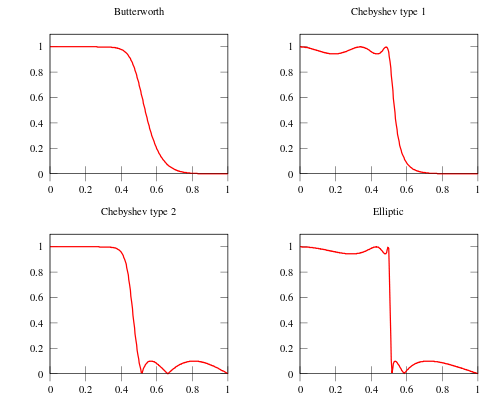
\includegraphics[width=0.6\textwidth]{figures/filtre}
\caption{De fire filtertyper; Butterworth, Cehbyshev 1 \& 2 og elliptisk}
\label{fig:filtre}
\end{figure}

Et Butterworth filter er karakteriseret ved ikke at have nogle rippels i hverken pasbåndet eller stopbåndet. Hertil er der, uanset filterorden, en dæmpning på 3 dB ved knækfrekvensen \citep{nilsson2015}.
Et Chebyshev filter har i modsætning til Butterworth et kortere transitionsbånd, som følge af en stejlere dæmpning, dog forekommer der ved et Chebyshev filter enten rippels i pasbåndet eller i stopbåndet. Ved et type 1 Chebyshev filter ses rippels i pasbåndet samt en monotont variation i stopbåndet. For type 2 Chebyshev ses der derimod rippels i stopbåndet og en monotont variation i pasbåndet \citep{nilsson2015}. 
Ved det elliptiske filter ses en endnu stejlere dæmning og dermed et kortere transitionsbånd end ved Butterworth samt Chebyshev filtre. Ved dette filter ses der dog både rippels i pasbånd og stopbånd \citep{nilsson2015}. 
